% XeLaTex
%\documentclass[review]{cvpr}
\documentclass[final]{cvpr}

\usepackage[UTF8]{ctex}

%\usepackage{cvpr}
\usepackage{times}
\usepackage{epsfig}
\usepackage{graphicx}
\usepackage{amsmath}
\usepackage{amssymb}
\usepackage{subfigure}
\usepackage{overpic}

\usepackage{url}
\usepackage{algorithm}
\usepackage{algorithmic}
\usepackage{siunitx}
\usepackage{amsmath}
\usepackage{amssymb}
\usepackage{booktabs}
\usepackage{float}
\usepackage{multirow}
% \usepackage{longtable}
\usepackage{array}
\usepackage[T1]{fontenc}
\usepackage[misc]{ifsym}
\usepackage{mathrsfs}
% for table
\usepackage{tabularx}

\usepackage{enumitem}
\setenumerate[1]{itemsep=0pt,partopsep=0pt,parsep=\parskip,topsep=5pt}
\setitemize[1]{itemsep=0pt,partopsep=0pt,parsep=\parskip,topsep=5pt}
\setdescription{itemsep=0pt,partopsep=0pt,parsep=\parskip,topsep=5pt}


\usepackage[pagebackref=true,breaklinks=true,colorlinks,bookmarks=false]{hyperref}


%\cvprfinalcopy % *** Uncomment this line for the final submission

\def\cvprPaperID{159} % *** Enter the CVPR Paper ID here
\def\confYear{CVPR 2020}
\def\httilde{\mbox{\tt\raisebox{-.5ex}{\symbol{126}}}}

\newcommand{\cmm}[1]{\textcolor[rgb]{0,0.6,0}{CMM: #1}}
\newcommand{\todo}[1]{{\textcolor{red}{\bf [#1]}}}
\newcommand{\alert}[1]{\textcolor[rgb]{.6,0,0}{#1}}

\newcommand{\IT}{IT}
\newcommand{\MZ}{MZ}
\newcommand{\GB}{GB}
\newcommand{\SR}{SR}
\newcommand{\FT}{FT}
\newcommand{\CA}{CA}
\newcommand{\LC}{LC}
\newcommand{\AC}{AC}
\newcommand{\HC}{HC-maps }
\newcommand{\RC}{RC-maps }
\newcommand{\Lab}{$L^*a^*b^*$}
\newcommand{\mypara}[1]{\paragraph{#1.}}

\floatname{algorithm}{算法}  
\renewcommand{\algorithmicrequire}{\textbf{输入:}}  
\renewcommand{\algorithmicensure}{\textbf{输出:}} 

\graphicspath{{figures/}}

% Pages are numbered in submission mode, and unnumbered in camera-ready
%\ifcvprfinal\pagestyle{empty}\fi
\setcounter{page}{1}

%%%%%%%%%%%%%%%%%%%%%%%%%%%%%%%%%%%%%%算法陈述可换页
\makeatletter
\newenvironment{breakablealgorithm}
  {% \begin{breakablealgorithm}
   \begin{center}
     \refstepcounter{algorithm}% New algorithm
     \hrule height.8pt depth0pt \kern2pt% \@fs@pre for \@fs@ruled
     \renewcommand{\caption}[2][\relax]{% Make a new \caption
       {\raggedright\textbf{\ALG@name~\thealgorithm} ##2\par}%
       \ifx\relax##1\relax % #1 is \relax
         \addcontentsline{loa}{algorithm}{\protect\numberline{\thealgorithm}##2}%
       \else % #1 is not \relax
         \addcontentsline{loa}{algorithm}{\protect\numberline{\thealgorithm}##1}%
       \fi
       \kern2pt\hrule\kern2pt
     }
  }{% \end{breakablealgorithm}
     \kern2pt\hrule\relax% \@fs@post for \@fs@ruled
   \end{center}
  }
\makeatother
%%%%%%%%%%%%%%%%%%%%%%%%%%%%%%%%%%%%%%

\begin{document}
% \begin{CJK*}{GBK}{song}

\renewcommand{\figref}[1]{图\ref{#1}}
\renewcommand{\tabref}[1]{表\ref{#1}}
\renewcommand{\equref}[1]{式\ref{#1}}
\renewcommand{\secref}[1]{第\ref{#1}节}
\def\abstract{\centerline{\large\bf 摘要} \vspace*{12pt} \it}

%%%%%%%%% TITLE

\title{简述图卷积神经网络\thanks{本文的编写基于CVPR'11论文
\cite{Cheng_SaliencyCvpr11}的\LaTeX 模板。}}
% \title{文献阅读报告\thanks{本文为CVPR'11论文
% \cite{Cheng_SaliencyCvpr11}的中文翻译版。}}

\author{柳明 \quad  \\
        School of CEI/AI,\;Nanjing Normal University\\
}

% \author{Ming-Ming Cheng$^{1}$\quad Guo-Xin Zhang$^{1}$ \quad Niloy J. Mitra$^{2}$
%     \quad Xiaolei Huang$^{3}$  \quad Shi-Min Hu$^{1}$  \\
%     $^{1}$ Tsinghua University \quad \quad
%     $^2$ KAUST   \quad \quad $^3$ Lehigh University\\
% }
%\thanks{本文的编写基于CVPR'11论文\cite{Cheng_SaliencyCvpr11}的$\LaTeX$模板。}
\maketitle
% \thispagestyle{empty}

%%%%%%%%% ABSTRACT
\begin{abstract}

卷积神经网络因其强大的建模能力引起研究者们的广泛关注,在图像处理、自然语言处理等领域得到了成功应用。然而,传统卷积神经网络只能处理欧式空间数据,而在许多应用场景如社交网络、交通网络、蛋白质网络中,数据都是以图数据的形式呈现的。本文首先介绍了图卷积神经网络的背景,之后就图卷积神经网络的两类主流方法展开简要叙述和梳理:谱方法基于谱图理论和卷积定理在谱域定义图卷积,空间方法通过直接在结点域定义结点相关性实现图卷积。最后,本文介绍了图卷积神经网络的相关应用,并对图卷积神经网络的发展做了一些总结。

\end{abstract}




%%%%%%%%% BODY TEXT %%%%%%%%%%%%%%%%%%%%%%%%%%%%%%%%%%%%%%%%


\section{引言}

卷积神经网络及其催生的一系列方法在过去近十年中得到了快速发展~\cite{he2016deep,ioffe2015batch,krizhevsky2012imagenet,simonyan2014very},它通过稀疏交互(sparse interactions)、参数共享(parameter sharing)、等变表示(equivariant representations)这三个重要的思想来帮助改进神经网络模型。卷积神经网络较全连接神经网络而言,通过减少连接数、共享参数等方法削弱了网络的表达能力上限,但使得整个网络更容易被训练。卷积神经网络在图像处理和自然语言处理等领域的一些具体问题上如机器翻译~\cite{hu2014convolutional}、图像识别~\cite{he2016deep}和语音识别~\cite{hinton2012deep}等表现出了强大的建模能力。

但是,传统的卷积神经网络只能处理欧式结构的数据(Euclidean data)如图像、文本等,这些领域的数据具有平移不变性。平移不变性(translation invariance) 使得我们可以在输入数据的数据空间定义全局共享的卷积核,从而定义卷积神经网络。以图像数据为例,一张图片可以表示为欧式空间一组网格状规则散布的像素点,那么平移不变性则表示以任意像素点为中心,可以获取到相同尺寸的局部结构。基于这些性质,卷积神经网络通过在训练过程中学习被每个像素点共享的卷积核参数(权重和偏置)来对局部连接进行建模,从而学习到丰富的隐层表示来体现图片的不同模式。

非欧式结构的数据广泛存在于科学研究和社会研究等领域,典型的例子有社交网络、交通网络、物体形状识别~\cite{mirbauer2021survey}的网状表面
(meshed surfaces)和通信的传感器网络等。这些例子中的数据都可以将其拓扑结构抽象为图数据,不同于图像和文本数据,对图中的每个结点来说,其局部结构都各不相同,这就使得此类数据不具有平移不变性~\cite{shuman2013emerging}。平移不变性的缺失对在图数据上重新定义卷积神经网络提出了挑战。

由于非欧数据的普遍性,越来越多的研究者尝试对已有的深度学习模型进行改造或类比已有方法、概念重新在图上定义某些操作,以满足对此类数据进行处理的需求。图数据上普遍存在的结点相邻和依赖关系与卷积神经网络对局部结构的强大建模能力让图卷积神经网络成为图深度学习领域相当活跃和重要的一个社区。在模式识别课程的文献阅读过程中,我们尝试结合几篇较有代表性的文章,在本文中对图卷积神经网络的发展历程进行一点简单的整理和总结。

\subsection{图卷积神经网络面临的挑战}
前面部分介绍过,图数据因为不满足平移不变性而难以直接用传统的卷积神经网络进行处理,除此以外,将卷积神经网络迁移到图数据上进行应用还存在其他难点。构建图卷积神经网络过程中的挑战主要来源于以下几个方面:
\mypara{图数据是非欧空间数据}
图数据作为非欧空间数据,不满足平移不变性,即每个结点的局部结构各异。传统卷积神经网络的两个基本算子(卷积和池化)都依赖于数据的平移不变性。如何在图数据上重新定义卷积和池化算子成为了首要的挑战性工作。
\mypara{图数据具有多样的特性}
实际生活中的多种场景都可以用图数据自然地表示,这使得这些具体场景下的图数据具有各种各样的特性,如社交网络中用户之间的有向连接,文献引用网络中作者和引文的异质连接,政治关系网络中的正负倾向带符号连接等。图的多样性使得图数据中蕴含的信息更加丰富,但是对多种特性进行建模也要求图卷积神经网络更加复杂精细,这也是图卷积神经网络面临的一个挑战。
\mypara{图数据的规模往往很大}
在实际的应用场景下,图的规模可能极大,含有百万甚至千万级别的结点,如推荐系统中的用户商品网络,社交网络中的用户网络。如何在可接受的空间和时间范围要求内,在大规模图数据上构建图卷积神经网络也是一大挑战。


\subsection{图卷积神经网络的任务}

图数据建模所针对的应用场景非常广泛,这也使得图数据建模所处理的任务也多种多样。对图数据建模可以求解图级别(graph-level)、结点级别(node-level)和边级别(edge-level)三种层面的问题。

图级别的任务可以描述为输入图数据,输出每个图的类别,包括图生成、图分类等,如蛋白质网络中的蛋白质分类、分子毒性预测。结点级别的任务的要求是输入结点不带类别的图,输出每个结点的级别,包括节点分类等,如引用网络中的文章分类。边级别的任务则用来预测结点之间的相互关系,包括链接预测(link prediction)等,如推荐系统中用户对商品的偏好推断。


\subsection{图卷积神经网络方法及分类}

图数据建模的历史由来已久。最初,研究人员更加关注统计分析的方法,如谷歌创始人提出的的网页排序算法PageRank~\cite{page1999pagerank}等,机器学习模型在初期并没有参与到图数据处理的发展中。此外,谱图理论(spectral graph theory)也常被应用到其中,如吴恩达等提出的谱聚类方法~\cite{ng2002spectral}可以用拉普拉斯矩阵的特征值和特征向量做社区分析或人群聚类等。随着近年来深度学习的崛起,研究者们也尝试将深度学习模型与图数据结合起来,这一阶段受Mikolov等提出的word2vec学习词嵌入~\cite{mikolov2013efficient}的启发,代表性的研究工作是图嵌入(graph embedding),即通过结点的邻近性为每个结点学习固定长度的低维、稠密的嵌入表示,如DeepWalk~\cite{perozzi2014deepwalk}、LINE~\cite{tang2015line}、node2vec~\cite{grover2016node2vec}等。这一时期,在解决具体的应用问题时,建模过程通常被分为两阶段:第一阶段,学习每个结点的统一长度的表示(即embedding);第二阶段,将学习到的结点表示作为输入,训练相应的分类模型。而近年来,研究重心也逐渐转移到如何将深度学习模型与图数据结合,直接进行端到端的学习。

图卷积神经网络的本质目的是用来提取拓扑图的空间特征,拓扑图源于从实际问题中抽取出的关系网络。实现这个目标有两种主流方式:最早提出的方法借助谱图理论将图上信息通过图傅里叶变换变换到谱域(spectral domain),结合卷积定理(convolution theorem)在谱域定义并实现卷积操作,谱方法的主要挑战是这样处理之后,定义在谱域的卷积核在空间上没有局部连接的性质;第二种方法是在空间域(spatial domain)或称顶点域(vertex domain)中直接提取邻居结点信息进行处理,空间方法将卷积算子重新定义为对目标顶点的邻居结点信息进行加权平均的函数,这种方法主要的挑战是不同结点的邻居数量可能差异巨大,例如有的图中顶点度数大致服从幂律分布(power-law degree distribution)。


% \subsection{分类}
%%%%%%%%%%%%%%%%%%%%%%%%%%%%%%%%%%%%%%%%%%%%%%%%%%%%%%%%%%%%%%%%%%%%%%%%%%%%%%%%%
\section{谱方法及基于谱方法的图卷积神经网络}
\label{sec:SpectralMethod}
图数据上平移不变性的确实,给在结点域定义卷积神经网络带来困难。谱方法基于谱图理论和卷积定理在谱域定于图卷积。本小节我们先介绍相关的背景知识和基本原理。

\subsection{谱方法的基本原理}
% \label{sec:BasicMethod}

为了便于后文叙述,首先我们在\tabref{tab:notation}中给出本文中一些常见符号及其基本含义。

\begin{table}[htb!]
    \centering
    \begin{tabular}{lccc} 
    \toprule
      符号  &  含义       \\ 
    \midrule
      $G$       &  图           \\
      $V$       &  结点集合     \\
      $E$       &  连边集合     \\
      $n$       &  结点个数     \\
      $\boldsymbol{I}_n \in R^{n \times n}$       &  单位矩阵     \\
      $\boldsymbol{A} \in R^{n \times n}$         &  邻接矩阵     \\
      $\boldsymbol{D} \in R^{n \times n}$         &  度矩阵(对角阵)     \\
      $\boldsymbol{L} \in R^{n \times n}$         &  拉普拉斯矩阵     \\
      $\boldsymbol{U} \in R^{n \times n}$         &  特征向量矩阵     \\
      $\boldsymbol{\Lambda} \in R^{n \times n}$   &  特征值矩阵(对角阵) \\
      $\boldsymbol{u}_i \in R^n$                  &  第$i$个特征向量     \\
      $\boldsymbol{X} \in R^{n \times d}$         &  结点特征矩阵     \\
      $\boldsymbol{X}_i \in R^d$                  &  第$i$个结点的特征     \\
      $\boldsymbol{f} \in R^n$                    &  信号     \\
    \bottomrule
    \end{tabular}
    \caption{符号定义。} \label{tab:notation}
\end{table}

我们用$G=\left( V,E,\boldsymbol{A} \right)$表示无向图,其中$V$表示图中结点组成的集合,$n = \left| V \right|$表示图上的结点数,$E$表示边集合,$\boldsymbol{A}$表示邻接矩阵,定义了结点之间的连接关系,且在无向图中有$\boldsymbol{A}_{i,j}=\boldsymbol{A}_{j,i}$。$\boldsymbol{D}$是图的度数矩阵,$\boldsymbol{D}_{i,i}$即为第$i$个结点的度且$\boldsymbol{D}_{i,i} = \sum_j \boldsymbol{A}_{i,j}$。

谱图理论中常用的拉普拉斯矩阵(Laplacian matrix)定义为$\boldsymbol{L} = \boldsymbol{D}-\boldsymbol{A}$。另外,在图表示学习领域,常用的拉普拉斯矩阵及其变体有三种。组合拉普拉斯矩阵(combinatorial Laplacian)即为刚才提到的由度数矩阵和邻接矩阵相减定义的形式$\boldsymbol{L} = \boldsymbol{D}-\boldsymbol{A}$;随机游走领域常用的随机游走归一化拉普拉斯矩阵(random walk normalized Laplacian)定义为
\begin{equation}
    \boldsymbol{L}^{rw} 
    = \boldsymbol{D}^{-1}\boldsymbol{L}
    = \boldsymbol{I}_n - \boldsymbol{D}^{-1}\boldsymbol{A}
\end{equation}
还有在图卷积神经网络领域应用广泛的对称规一化拉普拉斯矩阵(symmetric normalized Laplacian),定义为
\begin{equation}
    \boldsymbol{L}^{sys} 
    = \boldsymbol{D}^{-\frac{1}{2}}\boldsymbol{L}\boldsymbol{D}^{-\frac{1}{2}}
    = \boldsymbol{I}_n - 
    \boldsymbol{D}^{-\frac{1}{2}}\boldsymbol{A}\boldsymbol{D}^{-\frac{1}{2}}
\end{equation}
显然$\boldsymbol{L}$是一个实对称矩阵,可以被正交对角化,即对$\boldsymbol{L}$做特征分解$\boldsymbol{L}=\boldsymbol{U}\boldsymbol{\Lambda}\boldsymbol{U}^{\mathrm{T}}$,其中$\boldsymbol{U}=\left\{ \boldsymbol{u}_i \right\}_{i=1}^n
= \left[ \boldsymbol{u}_1,\cdots,\boldsymbol{u}_n \right]$表示$n$个相互正交的特征向量(eigenvector)组成的变换矩阵,$\boldsymbol{\Lambda}
= \mathrm{diag} \left[ \lambda_1,\cdots,\lambda_n \right] $是一个对角阵,$\lambda_i$表示与特征向量$\boldsymbol{u}_i$相对应的特征值。

$\boldsymbol{X}$表示图$G$上的结点特征(features),其中$\boldsymbol{X} \in R^{n \times d}$,每个结点有$d$个特征,行向量$\boldsymbol{X}_i \in R^d$是第$i$个结点的特征向量,列向量$\boldsymbol{x}_j \in R^n$表示图上结点的第$j$个特征(即为定义在结点上的一个信号),元素$\boldsymbol{X}_{i,j}$表示矩阵$\boldsymbol{X}$的第$i$行第$j$列,即第$i$个结点的第$j$个特征,$\boldsymbol{f},\boldsymbol{x},\boldsymbol{y} \in R^n$表示图上的信号,$\boldsymbol{f}_i$表示结点$i$在信号$\boldsymbol{f}$上的取值。

图信号处理领域的学者将传统信号处理中使用的的傅里叶变换(Fourier transform)推广到了图上~\cite{shuman2013emerging}。传统的傅里叶变换定义为
\begin{equation}
    F\left( \omega \right) = 
    \mathcal{F}\left[  f\left( t \right) \right] =
    \int f\left( t \right)e^{-i\omega t}dt
\end{equation}
即为信号$f\left( t \right)$与基函数$e^{-i\omega t}$乘积的积分。而时频傅里叶的基函数$e^{-i\omega t}$是拉普拉斯算子的特征函数,$\omega$和特征值有关。广义的特征方程定义为$AV=\lambda V$,其中$A$与本文中的邻接矩阵无关,只是一种变换,$V$是特征(eigen-)向量或特征函数,$\lambda$是特征值。函数$e^{-i\omega t}$满足
\begin{equation}
    \Delta e^{-i\omega t}
    =\frac{\partial ^2}
          {\partial t^2} e^{-i\omega t}
    =-\omega ^2 e^{-i\omega t}
\end{equation}
根据广义的特征方程定义,$e^{-i\omega t}$就是$\Delta$的特征函数。

在谱图理论~\cite{chung1997spectral}中有这样一个结论:一个图的拉普拉斯矩阵,就等价于定义在这个图上的拉普拉斯算子(二阶微分)。那么回到广义特征方程$AV=\lambda V$,用拉普拉斯矩阵$\boldsymbol{L}$代替变换$A$,得到$\boldsymbol{L}V=\lambda V$。类比时频傅里叶的推导过程,我们就可以用拉普拉斯矩阵的特征向量作为图傅里叶变换的基。以拉普拉斯矩阵的特征向量作为谱空间下一组基底,那么图上信号$\boldsymbol{x} \in R^n$的傅里叶变换为
\begin{equation}\label{equ:graph-Fourier-1}
    \hat{\boldsymbol{x}} =
    \boldsymbol{U}^{\mathrm{T}}\boldsymbol{x}
\end{equation}
其中,$\boldsymbol{x}$为信号在结点域的原始表示,$\hat{\boldsymbol{x}}$为信号$\boldsymbol{x}$变换到谱域之后的表示,$\boldsymbol{U}^{\mathrm{T}}$表示特征向量矩阵的转置,用于做傅里叶变换。同样,信号$\boldsymbol{x}$的傅里叶逆变换为
\begin{equation}\label{equ:graph-Fourier-2}
    \boldsymbol{x} =
    \boldsymbol{U}\hat{\boldsymbol{x}}
\end{equation}

在此基础上,谱方法利用卷积定理在谱域上定义了图卷积。关于卷积定理可以叙述为:信号卷积的傅里叶变换等价于信号傅里叶变换后的乘积,形式化描述为
\begin{equation}\label{equ:conv-theorem}
    \mathcal{F} \left( \boldsymbol{x}*\boldsymbol{y} \right)
    =
    \mathcal{F} \left( \boldsymbol{x} \right) \cdot 
    \mathcal{F} \left( \boldsymbol{y} \right)
\end{equation}
其中,$\boldsymbol{x}$和$\boldsymbol{y}$表示两个原始信号,$*$表示卷积算子,$\cdot$表示乘积算子。对式\ref{equ:conv-theorem}等号两侧同时做傅里叶逆变换,可以得到
\begin{equation}\label{equ:conv-theorem-ada}
    \boldsymbol{x}*\boldsymbol{y}
    =
    \mathcal{F}^{-1} \left( \mathcal{F} \left( \boldsymbol{x} \right) \cdot 
    \mathcal{F} \left( \boldsymbol{y} \right) \right)
\end{equation}
其中,$\mathcal{F}^{-1}\left( \boldsymbol{x} \right)$表示信号$\boldsymbol{x}$的傅里叶逆变换。

根据以上理论基础,由式\ref{equ:graph-Fourier-1}、式\ref{equ:graph-Fourier-2}和式\ref{equ:conv-theorem-ada},可将图上的卷积写为
\begin{equation}\label{equ:graph-conv}
    \boldsymbol{x}*_{G}\boldsymbol{y}=\boldsymbol{U}
    \left(
        \left(
            \boldsymbol{U}^{\mathrm{T}}\boldsymbol{x}
        \right)
        \odot 
        \left(
            \boldsymbol{U}^{\mathrm{T}}\boldsymbol{y}
        \right)          
    \right)
\end{equation}
其中,$*_G$表示图上的卷积算子,$\odot $为哈达玛积(Hadamard product)即将向量、矩阵对应位置元素相乘,可以将信号$\boldsymbol{x}$视为输入信号,信号$\boldsymbol{y}$视为卷积核,在谱空间的卷积核是$\boldsymbol{U}^{\mathrm{T}}\boldsymbol{y}$。

我们令$\boldsymbol{U}^{\mathrm{T}}\boldsymbol{y}=\left[ \theta_0,\cdots,\theta_{n-1} \right]^{\mathrm{T}} $,$g_{\theta}=\mathrm{diag} \left( \left[ \theta_0,\cdots,\theta_{n-1} \right]  \right)
$,那么就可以用对角阵$g_{\theta}$代替列向量$\boldsymbol{U}^{\mathrm{T}}\boldsymbol{y}$,之后就可以将哈达玛积运算转化为简洁的矩阵乘法形式,从而将式\ref{equ:graph-conv}化成
\begin{equation}\label{equ:graph-conv-ada}
    \boldsymbol{x}*_{G}\boldsymbol{y}=\boldsymbol{U}
    g_{\theta}
    \boldsymbol{U}^{\mathrm{T}}\boldsymbol{x}      
\end{equation}

经过以上推导,我们得到了图上卷积算子的定义,基于此定义,谱方法一支陆续出现了一些图卷积神经网络模型。


\subsection{基于谱方法的图卷积神经网络}
本小节基于前述的基本原理简单介绍几个具有代表性的基于谱方法的图卷积神经网络工作。
\mypara{Spectral CNN}
谱卷积神经网络(Spectral CNN)~\cite{bruna2014spectral}由LeCun组的Bruna等人在2014年提出,是最早被提出的构建图卷积神经网络的方法,他们从基本的谱图理论出发并结合卷积定理,在谱空间定义了图卷积。该方法利用卷积定理在每一层定义图卷积算子,并堆叠多层组成神经网络。

\begin{figure}[htb!]
    \centering
    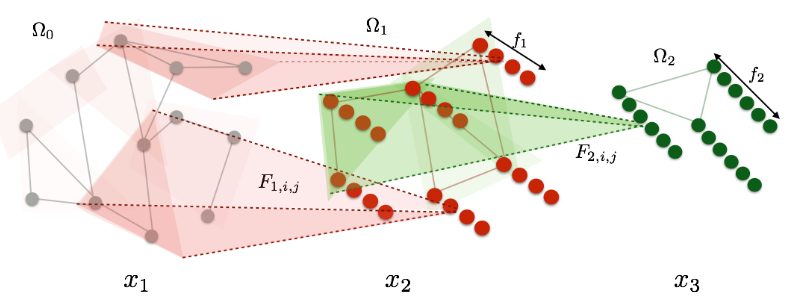
\includegraphics[width=0.75\textwidth]{Spectral CNN.png}
    \caption{谱卷积神经网络。}
    \label{fig:Spectral CNN}
\end{figure}

谱卷积神经网络第$m$层的前向传播过程(公式和符号等均采用本文记法,与原文中有不同)如下
\begin{equation}\label{equ:spectral-cnn-forward}
    \boldsymbol{x}_j^{m+1}=
    h \left(
        \boldsymbol{U}
        \sum_{i=1}^{p}
        F_{i,j}^m 
        \boldsymbol{U}^{\mathrm{T}}
        \boldsymbol{x}_i^{m}
    \right), \quad j=1,\cdots,q
\end{equation}
其中,$p$和$q$分别是输入特征(features)和输出特征的维度,即第$m$层和第$m+1$层的通道数,$\boldsymbol{x}_i^{m} \in R^n$表示图上结点在第$m$层的第$i$个输入特征,$F_{i,j}^m$表示谱空间下第$m$层的可学习的卷积核,是一个对角阵,$h$表示非线性激活函数。在谱卷积神经网络中,这样一层结构将特征(features)从$p$维转化到$q$维,且基于卷积定理通过学习卷积核的参数实现了图卷积。

总的来说,谱卷积神经网络将卷积核作用在谱空间的输入信号上,并利用卷积定理实现图卷积,以完成结点之间的信息聚合,然后将非线性激活函数作用在信息聚合的结果上,堆叠多层形成神经网络。但是,谱卷积神经网络也存在一些缺陷:首先,谱卷积神经网络方法要求对图的拉普拉斯矩阵进行特征分解(eigen-decomposition),因为图卷积的求解过程中显式地使用了拉普拉斯矩阵的特征向量,并且每一次前向传播,都要计算$\boldsymbol{U}$、卷积核(对角阵)和$\boldsymbol{U}^{\mathrm{T}}$三者的矩阵乘积,计算代价非常高,论文中也提到这会有$O \left( n^3 \right)$的计算复杂度;其次,卷积核有$n$个参数,而数$n$直接受到图规模的影响,尤其对于大规模图来说;最后,谱卷积神经网络不满足局部连接(spatial localization)的性质,因为卷积核作用在信号$\boldsymbol{x}_i$上,而信号$\boldsymbol{x}_i$含有全部结点第$i$个特征的信息,意味着每次信息聚合其实都有全局信息的参与。

\mypara{ChebNet} 
Spectral CNN提出之后出现了一些工作致力于实现图卷积神经网络的局部性和加速计算,Defferrard等人提出的切比雪夫网络(ChebNet)~\cite{defferrard2016convolutional}通过参数化卷积核实现局部性,也降低了参数复杂度和计算复杂度。

在式\ref{equ:graph-conv-ada}中,$g_{\theta}$是需要学习的卷积核,在谱卷积神经网络中,$g_{\theta}$是一个有$n$个待学习参数的对角阵。Defferrard等在文章中提出,对于卷积核$g_{\theta}$,我们如果对其用一个$K$阶多项式进行拟合:
\begin{equation}\label{equ:chebnet-polynomial}
    g_{\beta}\left( \boldsymbol{\Lambda} \right)
    \approx \sum_{k=0}^{K-1} \beta_k
    \boldsymbol{\Lambda}^k
\end{equation}
其中,$\Lambda=\mathrm{diag}\left( \lambda_1,\lambda_2,\cdots,\lambda_n \right)$。将式\ref{equ:chebnet-polynomial}代入式\ref{equ:graph-conv-ada},图卷积可化为
\begin{align}
    \boldsymbol{x} *_G \boldsymbol{y}
    &= \boldsymbol{U}
    g_{\beta}\left( \boldsymbol{\Lambda} \right)
    \boldsymbol{U}^{\mathrm{T}}\boldsymbol{x} \notag \\
    &=\boldsymbol{U} \sum_{k=0}^{K-1} \beta_k \boldsymbol{\Lambda}^k
    \boldsymbol{U}^{\mathrm{T}}\boldsymbol{x} \notag \\
    &=\sum_{k=0}^{K-1} \beta_k
    \left( \boldsymbol{U} \boldsymbol{\Lambda}^k
    \boldsymbol{U}^{\mathrm{T}}
    \right) \boldsymbol{x} \notag \\
    &=\sum_{k=0}^{K-1} \beta_k
    \boldsymbol{L}^k
    \boldsymbol{x} \label{equ:chebnet-poly-graph-conv}
\end{align}
这样就将参数个数从$n$个减少到$K$个,一般$K$远远小于$n$;同时也不需要进行矩阵的特征分解,之前用傅里叶变换的基$\boldsymbol{U}^{\mathrm{T}}$乘信号$\boldsymbol{x}$的计算复杂度是$O \left( n^2 \right)$,而现在由于式\ref{equ:chebnet-poly-graph-conv}中拉普拉斯矩阵$\boldsymbol{L}$是一个比较稀疏的矩阵,这一步的运算量与结点数$n$无关,只和边数有关,所以这一步的计算复杂度可以被降低到$O \left( \left| E \right|\right)$。

具体地,ChebNet引入了切比雪夫多项式(Chebyshev polynomial)$T_k$对$g_\theta$进行拟合。切比雪夫多项式的递推定义为
\begin{equation}\label{equ:cheb-poly-def}
\left\{
    \begin{array}{lr}
        T_0 \left( x \right) = 1 &\\  
        T_1 \left( x \right) = x &\\  
        T_k \left( x \right) = 2xT_{k-1} \left( x \right) 
        -T_{k-2} \left( x \right) &
    \end{array}
\right.
\end{equation}
$g_\beta$的$K$阶近似为
\begin{equation}\label{equ:g-beta-approx}
    g_{\beta}\left( \boldsymbol{\Lambda} \right)
    \approx \sum_{k=0}^{K-1} \beta_k
    T_k \left( \widetilde{\boldsymbol{\Lambda}} \right)
\end{equation}
其中,$\widetilde{\boldsymbol{\Lambda}}=2\boldsymbol{\Lambda} / \lambda_{max} - \boldsymbol{I}_n$,$\lambda_{max}$是拉普拉斯矩阵最大的特征值,拉普拉斯矩阵是半正定矩阵,其特征值都非负(有特征值0),这个操作将特征值压缩到$\left[ -1,1 \right]$的范围中,可以防止梯度爆炸。
那么根据式\ref{equ:g-beta-approx}和式\ref{equ:graph-conv-ada},我们可以将切比雪夫多项式代入化简,具体地,图卷积可以写成
\begin{align}
    \boldsymbol{x} *_G \boldsymbol{y}
    &= \boldsymbol{U}
    g_{\beta}\left( \boldsymbol{\Lambda} \right)
    \boldsymbol{U}^{\mathrm{T}}\boldsymbol{x} \notag \\
    &=\boldsymbol{U} \sum_{k=0}^{K-1} \beta_k T_k ( \widetilde{\boldsymbol{\Lambda}} )
    \boldsymbol{U}^{\mathrm{T}}\boldsymbol{x} \notag \\
    &=\sum_{k=0}^{K-1} \beta_k
    \left( \boldsymbol{U} T_k ( \widetilde{\boldsymbol{\Lambda}} )
    \boldsymbol{U}^{\mathrm{T}}
    \right) \boldsymbol{x} \notag \\
    &=\sum_{k=0}^{K-1} \beta_k
    T_k ( \boldsymbol{U} \widetilde{\boldsymbol{\Lambda}} 
    \boldsymbol{U}^{\mathrm{T}} )
    \boldsymbol{x} \notag \\    
    &=\sum_{k=0}^{K-1} \beta_k
    T_k ( \widetilde{\boldsymbol{L}} )
    \boldsymbol{x} \label{equ:chebnet-poly-graph-conv-spec}
\end{align}
其中,和$\widetilde{\boldsymbol{\Lambda}}$类似地有$\widetilde{\boldsymbol{L}}=2\boldsymbol{L} / \lambda_{max} -     \boldsymbol{I}_n$。式\ref{equ:chebnet-poly-graph-conv-spec}中第三步到第四步的推导$\boldsymbol{U} T_k ( \widetilde{\boldsymbol{\Lambda}} )
\boldsymbol{U}^{\mathrm{T}}=T_k ( \boldsymbol{U}
\widetilde{\boldsymbol{\Lambda}} \boldsymbol{U}^{\mathrm{T}})
$用数学归纳法可以很容易证得。

基于以上内容,切比雪夫网络第$m$层的前向传播过程可以记为
\begin{align}
    \boldsymbol{x}_j^{m+1}
    &=
    h \left(
        \boldsymbol{U}
        \sum_{i=1}^{p}
        \left(
        \sum_{k=0}^{K-1} \beta_k
        T_k ( \widetilde{\boldsymbol{\Lambda}} )
        \right)
        \boldsymbol{U}^{\mathrm{T}}
        \boldsymbol{x}_i^{m}
    \right),  \notag \\
    &= 
    h \left(
        \sum_{i=1}^{p}
        \sum_{k=0}^{K-1} \beta_k
        T_k ( \widetilde{\boldsymbol{L}} )
        \boldsymbol{x}_i^{m}
    \right)
    ,\quad j=1,\cdots,q  \label{equ:chebnet-forward}
\end{align}
与前文记法相同,$p$和$q$分别是输入特征(features)和输出特征的维度,即第$m$层和第$m+1$层的通道数,$\boldsymbol{x}_i^{m} \in R^n$表示图上结点在第$m$层的第$i$个输入特征,$h$表示非线性激活函数。

切比雪夫网络利用特征值矩阵的多项式参数化卷积核实现了谱卷积神经网络,而且巧妙地利用了$\boldsymbol{L}=\boldsymbol{U}\boldsymbol{\Lambda}\boldsymbol{U}^{\mathrm{T}}$的关系引入拉普拉斯矩阵,从而避免了对拉普拉斯矩阵的特征分解,同时参数的复杂度从$O \left( n \times p \times q \right)$下降到$O \left( K \times p \times q \right)$。

此外,参数化的卷积核很好地保证了局部性,式\ref{equ:chebnet-poly-graph-conv}中的$\boldsymbol{L}^k$就体现了局部连接特性,在拉普拉斯矩阵中,当且仅当结点$i,j$满足$K$跳可达时,$\boldsymbol{L}_{i,j}^K \neq 0$,这里和离散数学或图论中提到过的邻接矩阵$k$次幂的意义类似,代表着$k$阶可达关系。特别地,$K$就控制着卷积核的感受野(receptive field)大小,也就是说每次卷积会将距离中心顶点$K$跳之内的所有邻居上的特征(features)信息进行加权求和,权值就是在模型中学习的参数$\beta_k$。$K=1$和$K=2$的情形如图\ref{fig:chebnet-1}和图\ref{fig:chebnet-2}所示。
\begin{figure}[htb!]
    \centering
    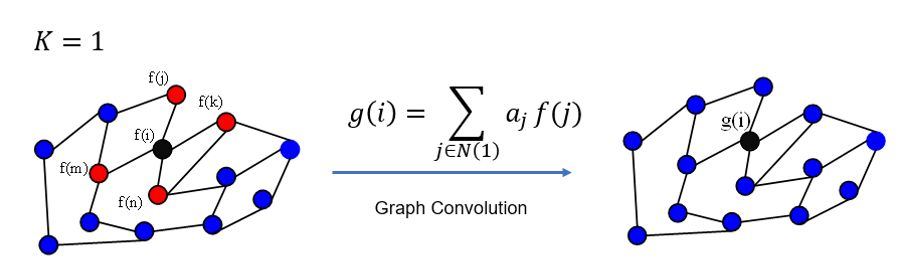
\includegraphics[width=0.63\textwidth]{chebnet-1.jpg}
    \caption{切比雪夫网络$K=1$时的图卷积示意。}
    \label{fig:chebnet-1}
\end{figure}
\begin{figure}[htb!]
    \centering
    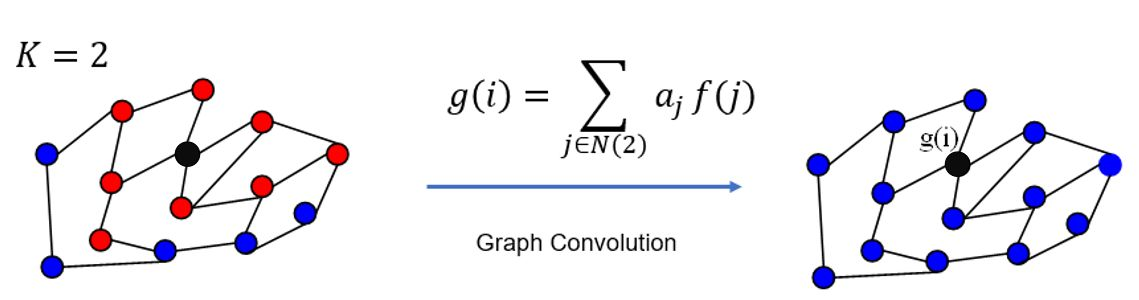
\includegraphics[width=0.63\textwidth]{chebnet-2.jpg}
    \caption{切比雪夫网络$K=2$时的图卷积示意。}
    \label{fig:chebnet-2}
\end{figure}


\mypara{Graph Wavelet Neural Network} 
图小波神经网络~\cite{xu2018graph}由中科院计算所徐冰冰等人在ICLR 2019上发表,不同于切比雪夫网络对谱卷积神经网络中的卷积核进行多项式参数化而达到实现局部性和加速计算的方式,小波神经网络更换了傅里叶变换的基底,用小波变换代替傅里叶变换,同样也满足了局部性和加速计算的要求。

小波神经网络指出,小波变换也定义了一种将信号从结点域变换到谱域的方法~\cite{hammond2011wavelets}。这里用
\begin{equation}
\boldsymbol{\Psi}_s=\left\{ \psi_{s1},\psi_{s2},\cdots,\psi_{sn} \right\}
\end{equation}
表示小波变换的基底,其中$\psi_{si}$表示从第$i$个结点出发的能量扩散,刻画了第$i$个结点的局部结构。小波基底的定义依赖于拉普拉斯矩阵的特征向量,即$\boldsymbol{\Psi}_s=\boldsymbol{U} \boldsymbol{G}_s \boldsymbol{U}^{\mathrm{T}}$,其中$\boldsymbol{G}_s= \mathrm{diag} \left( \left\{ g_s(\lambda_i) \right\}_{i=1}^n \right) $,对角线元素由$g$函数作用在特征值上得到。选取不同的$g$函数会赋予小波基底不同的性质,在小波神经网络中,作者使用了热核(heat kernel)函数,即$g_s(\lambda_i)=e^{s \lambda_i}$。

以$\boldsymbol{\Psi}_s$为谱空间的基底,则图上小波逆变换的变换矩阵为$\boldsymbol{\Psi}_s^{-1}=\boldsymbol{U} \boldsymbol{G}_{-s} \boldsymbol{U}^{\mathrm{T}}$,其中$\boldsymbol{G}_{-s}$表示将上述$g$函数替换为$g_{-s}(\lambda_i)=e^{-s \lambda_i}$。

那么,图卷积的定义式\ref{equ:graph-conv}可以被改写成
\begin{equation}\label{equ:gwnn-graph-conv}
    \boldsymbol{x}*_{G}\boldsymbol{y}={\Psi}
    \left(
        \left(
            \boldsymbol{\Psi}^{-1}\boldsymbol{x}
        \right)
        \odot 
        \left(
            \boldsymbol{\Psi}^{-1}\boldsymbol{y}
        \right)          
    \right)
\end{equation}

图小波神经网络第$m$层的前向传播过程可以记为
\begin{equation}\label{equ:gwnn-forward}
    \boldsymbol{x}_j^{m+1}=
    h \left(
        \boldsymbol{\Psi}_s
        \sum_{i=1}^{p}
        F_{i,j}^m 
        \boldsymbol{\Psi}_s^{-1}
        \boldsymbol{x}_i^{m}
    \right), \quad j=1,\cdots,q
\end{equation}
同样地,$p$和$q$分别是输入特征(features)和输出特征的维度,$\boldsymbol{x}_i^{m} \in R^n$表示图上结点在第$m$层的第$i$个输入特征,$F_{i,j}^m$表示谱空间下第$m$层的可学习的卷积核,是一个对角阵,$h$表示非线性激活函数。

由式\ref{equ:gwnn-forward}可以看出,在定义的图小波神经网络中,每层的参数的复杂度为$O \left( n \times p \times q \right)$,其中$n$是结点数,$p$是当前层中每个顶点的特征(feature)数,$q$是下一层中每个顶点的特征数。大量的自由参数需要更大数据量的训练数据来学习,会对网络的表达能力造成影响,针对这个缺陷,作者提出可以对原先的卷积操作操作进行解耦,分解为特征变换和图卷积两步:
\begin{align}
    &\mathrm{feature\;transformation:\;} 
    \boldsymbol{X}^{m'} =
    \boldsymbol{X}^{m}\boldsymbol{W} \label{gwnn-detach-1} 
    \\
    &\mathrm{graph\;convolution:\;} 
    \boldsymbol{X}^{m+1} =
    h \left(
    \boldsymbol{\Psi}_s \boldsymbol{F}^m
    \boldsymbol{\Psi}_s^{-1}\boldsymbol{X}^{m'}
    \right) \label{gwnn-detach-2} 
\end{align}
其中,$\boldsymbol{W} \in R^{p \times q}$是特征变换矩阵,$\boldsymbol{X}^{m} \in R^{n \times p}$为第$m$层的输入张量(tensor),$\boldsymbol{X}^{m+1} \in R^{n \times q}$为第$m$层的输出张量,$\boldsymbol{F}^m$是图卷积核(对角阵)。这个解耦方法有效减少了参数量,将参数复杂度从$O \left( n \times p \times q \right)$降低到了$O \left( n + p \times q \right)$,保持了模型较好的表达能力。

和傅里叶变换相比,小波基底具有一些很好的性质:(1)小波变换的基底可以通过切比雪夫多项式近似得到,也可以避免拉普拉斯矩阵特征分解带来的高计算代价;(2)小波变换的基底有局部性;(3)小波基底的局部性使得小波变换矩阵非常系数,大大降低了$\boldsymbol{\Psi}_s^{-1} \boldsymbol{x}$的计算复杂度;(4)热核函数中的超参数$s$表示热量扩散的范围,通过调节超参数$s$可以灵活地让小波网络适应于不同的任务场景。不同$s$值下的小波变换基底如图\ref{fig:GWNN-heatkernel}所示。图\ref{fig:GWNN-heatkernel}中左图表示在$s$较小时,以黄色结点为中心进行的热量扩散;右图表示当$s$增大时,热量扩散范围也变大。

\begin{figure}[htb!]
    \centering
    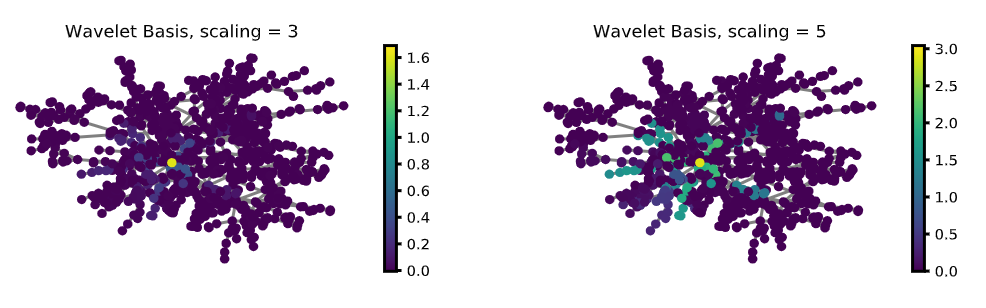
\includegraphics[width=0.85\textwidth]{GWNN-heatkernel.png}
    \caption{不同$s$值下的小波变换基底。}
    \label{fig:GWNN-heatkernel}
\end{figure}

文中~\cite{xu2018graph}也在顶点分类任务的3个数据集上对比了小波神经网络与其他方法。具体结果如表\ref{tab:GWNN-bench}所示,可以看出图小波神经网络的效果较优于其他谱方法。
\begin{table}[htb!]
    \centering
    \begin{tabular}{lcccccc} 
    \toprule
        \textbf{Method}  &  \textbf{Cora}   &  \textbf{Citeseer}  &   \textbf{Pumbmed} \\ 
    \midrule
        MLP & $55.1\%$   & $46.5\%$  & $71.4\%$ \\ 
        ManiReg & $59.5\%$   & $60.1\%$  & $70.7\%$ \\
        DeepWalk & $67.2\%$   & $43.2\%$  & $65.3\%$ \\
        ICA & $75.1\%$   & $69.1\%$  & $73.9\%$ \\
    \midrule
        Spectral CNN & $73.3\%$   & $58.9\%$  & $73.9\%$ \\ 
        ChebNet & $81.2\%$   & $69.8\%$  & $74.4\%$ \\ 
        GCN & $81.5\%$   & $70.3\%$  & $79.0\%$ \\ 
        MoNet & $81.7\pm 0.5 \%$   & $——$  & $78.8\pm 0.3 \%$ \\ 
    \midrule
        GWNN & $\textbf{82.8\%}$ & $\textbf{71.7\%}$ & $\textbf{79.1\%}$ \\
    \bottomrule
    \end{tabular}
    \caption{GWNN在顶点分类任务上的结果。}\label{tab:GWNN-bench}
\end{table}


% \begin{figure}[htb!]
%     \centering
%     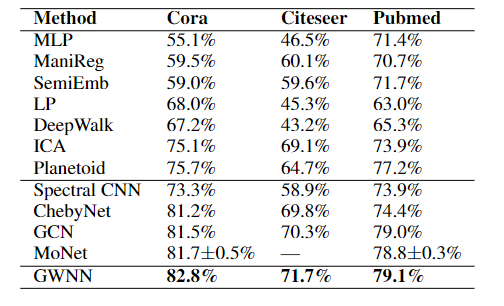
\includegraphics[width=0.55\textwidth]{GWNN-benchmark.png}
%     \caption{GWNN在顶点分类任务上的结果。}
%     \label{fig:GWNN-benchmark}
% \end{figure}
%%%%%%%%%%%%%%%%%%%%%%%%%%%%%%%%%%%%%%%%%%%%%%%%%%%%%%%%%%%%%%%%%%%%%%%%%%%%%%%%%
\section{空间方法及基于空间方法的图卷积神经网络}

上述方法都是从卷积定理出发在谱域定义图卷积,空间方法旨在从结点域出发,通过在结点域上直接定义聚合函数(aggregator)来聚合每个中心结点和它的邻近结点的信息,例如切比雪夫网络等可以视为以拉普拉斯矩阵或其变体形式作为聚合函数。在此启发下,开始出现一些工作通过注意力机制或其他方法直接从结点域学习聚合函数。此外,也有一部分工作通过类似传统卷积神经网络的工作方式,从空间角度定义了图卷积神经网络的通用框架并尝试解释图卷积神经网络的内部机制。
\label{sec:SpatialMethod}
\subsection{空间方法的基本原理} 
Niepert等人在2016年提出了一种可以在任意图上构造卷积神经网络的通用框架~\cite{niepert2016learning},在论文中作者对传统卷积神经网络在图片(image)上的工作流程进行拆解,重新审视了传统的卷积过程,通过类比的方法将卷积过程重新在结点域上定义。下面本小节以此为代表对空间方法的基本思路进行简单的介绍。

图\ref{fig:learn-conv-for-graph-1}中描述了一个大小为$3 \times 3$的卷积核在$4 \times 4$的图片上滑动的过程。作者将传统卷积神经网络中的卷积操作分解为3个步骤进行分析:(1)确定中心结点的若干个邻居结点,图片是由规整排列的像素点构成的,可以看做是一种网格化(grid-like)的图,在示例图中,卷积核窗口里就包括了中心结点(图中标红)及其邻居;(2)给中心结点的若干个邻居结点确定一个顺序,在传统卷积神经网络中我们并未考虑过这一步,因为图片的像素点是自然有序的,或者说大家都默认了这样一种从左到右、从上到下的定序方式;(3)参数共享是卷积神经网络中的重要机制,以图\ref{fig:learn-conv-for-graph-1}中过程为例,$3 \times 3$的卷积核每次都对原图像上同样$3 \times 3$大小的一个局部区域进行特征提取,这些局部区域中,位置相同的像素结点(如
每次滑动处理时的中心结点,在图中标注了序号)在进行计算的时候的权值和偏置是共享的。

\begin{figure}[htb!]
    \centering
    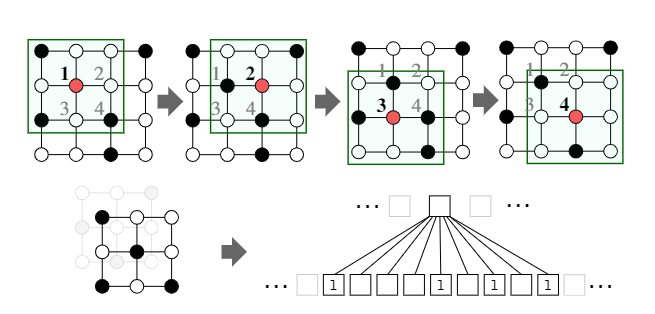
\includegraphics[width=0.65\textwidth]{learn-conv-for-graph-1.png}
    \caption{一个卷积核大小为$3 \times 3$的传统卷积神经网络。(步长为1,无填充)}
    \label{fig:learn-conv-for-graph-1}
\end{figure}


为了更好地类比传统卷积神经网络的工作流程和图数据上的操作,我们再将这3个步骤都放到处理图数据的情景下进行分析:(1)在实际应用场景下的图数据上,每个结点的连接性可能差异非常大,有的结点邻居非常多而有的只和很少一些结点相连;(2)对提取出的结点进行定序也是一个需要解决的问题,不像图片有着天生的规整结构,在图数据中每次提取出的子图是形态各异的,这也要求研究者采取一些规则化的定序方法;(3)关于参数共享也是和第一步有相同的难处,如果前一个窗口中中心结点a的邻居个数为10,后一个窗口中相对应的中心结点b却有10000个邻居,显然不可能直接让它们之间共享参数,但只要能够完成确定邻居、提取子图再定序的步骤,参数共享这一步工作也自然水到渠成。

\begin{figure}[htb!]
    \centering
    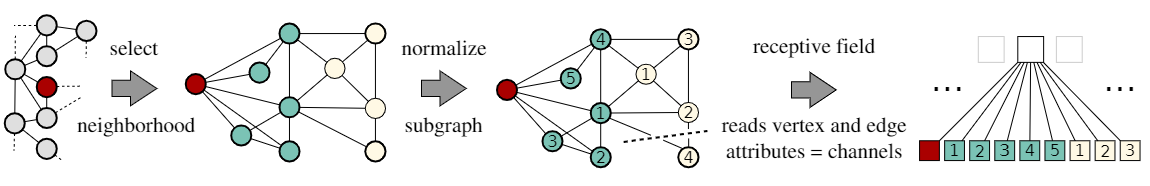
\includegraphics[width=0.96\textwidth]{learn-conv-for-graph-2.png}
    \caption{将卷积操作解构之后迁移到图上。}
    \label{fig:learn-conv-for-graph-2}
\end{figure}

作者提出的方法大致思路如图\ref{fig:learn-conv-for-graph-2}中所示。首先,对每个中心结点,都选取$k-1$($k$是超参数)个邻居结点,从而提取出的一个大小为$k$的邻域集合;对于定序,可以根据具体任务选择不同的相似性度量,例如根据结点的度定序、根据到中心结点的跳数定序等度量方式;最后,就得到了长度为$k$的一个有序序列,这样就可以直接用经典卷积神经网络的工具进行处理,其中边的属性和顶点的属性对应不同的输入通道。

基于此类思路,有更多的基于空间方法的图卷积神经网络被提出。


\subsection{基于空间方法的图卷积神经网络}
本小节基于前述的基本原理简单介绍几个具有代表性的基于空间方法的图卷积神经网络工作。

\mypara{GraphSAGE}
图采样聚合网络~\cite{hamilton2017inductive}在2017年由Hamilton等人提出,其中“SAGE”也就直接概括了该模型对数据的处理方法:采样和聚合(SAmple and aggreGatE)。不同于之前许多模型考虑所有邻近结点的做法,图采样聚合网络采取的策略是对邻近结点做随机采样,使每个结点的邻近结点都不多于给定的采样个数。
图采样聚合网络的结构和工作流程如图\ref{fig:graphSAGE}所示。以正红色结点为目标结点,图采样聚合网络首先对其一阶邻居和二阶邻居做随机采样,并仅把采样到的结点作为相关结点,然后模型将聚合函数作用在相关结点的特征表达上,并用聚合结果更新目标结点的特征表达来完成对应任务。

其中,先对邻近结点进行随机采样可以降低计算的复杂度(图中一阶邻居采样数为3,二阶邻居采样数为5)。此外,聚合步骤并不是直接聚合所有的一阶邻居和二阶邻居,而是先聚合二阶邻居的特征信息得到一阶邻居的特征表示,再聚合一阶邻居的信息最后得到目标结点的特征表示。


\begin{figure}[htb!]
    \centering
    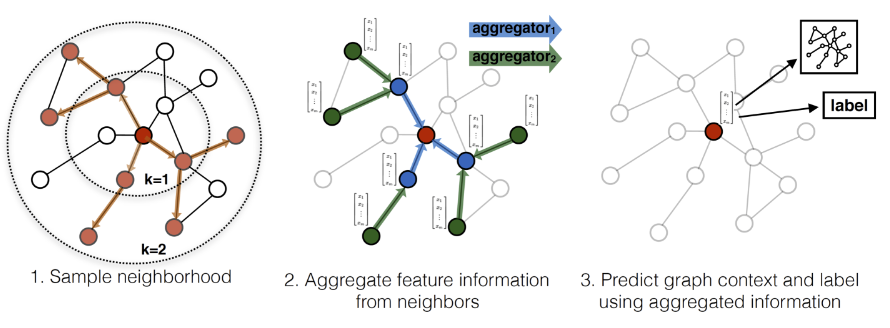
\includegraphics[width=0.76\textwidth]{graphSAGE.png}
    \caption{图采样聚合网络。}
    \label{fig:graphSAGE}
\end{figure}

其中,作者们给出了多种聚合函数的形式,分别是基于最大值的聚合,基于均值的聚合和基于长短时记忆网络(LSTM)~\cite{hochreiter1997long}的聚合。最大值聚合和均值聚合类似卷积中的最大池化(max pooling)和平均池化(average pooling),取相关结点的最大值和均值作为聚合结果(逐个特征);基于长短时记忆网络的聚合指将相关结点的embedding输入LSTM,把LSTM的输出作为聚合的结果,但显然虽然LSTM聚合表达能力更强,但是LSTM的学习过程会受到输入序列顺序的影响,所以输入LSTM进行聚合之前需要将相关结点随机排列打乱顺序,以便让模型适应无序的输入集合。

图采样聚合网络可以做归纳学习(inductive learning),可以对训练过程中见不到的数据直接计算而不需要重新对整个图进行学习,扩大了图神经网络的落地场景。另外,图采样聚合网络的预测速度非常快,因为实现中的随机采样使它只需要选择若干跳范围内的若干个邻居即可,并且原理并不复杂,不需要复杂的理论基础也能理解。

值得一提的是,2018年斯坦福和Pinterest公司合作提出了第一个工业级别(数十亿节点和数百亿边)基于图卷积神经网络的推荐系统PinSage~\cite{ying2018graph},并在离线评估和AB实验选中取得了不错的效果,这也是图卷积神经网络在商业推荐系统首次得到成功应用。


\mypara{Graph Convolution Network} 
为了使图卷积神经网络能够适应图上半监督学习领域的任务,Kipf等人\cite{kipf2016semi}对切比雪夫网络进行简化并提出了GCN(为防止混淆可以称为一阶图卷积神经网络),他们在文中令$K=2$且$\lambda_{max}=2$,将式\ref{equ:chebnet-forward}写为
\begin{align}
    \boldsymbol{x}_j^{m+1}
    &= 
    h \left(
        \sum_{i=1}^{p}
        \sum_{k=0}^{K-1} \beta_k
        T_k ( \widetilde{\boldsymbol{L}} )
        \boldsymbol{x}_i^{m}
    \right) \notag \\
    &= 
    h \left(
        \sum_{i=1}^{p}
        \left(
        \beta_0 T_0 ( \widetilde{\boldsymbol{L}} )+
        \beta_1 T_1 ( \widetilde{\boldsymbol{L}} )
        \right) \boldsymbol{x}_i^{m}
    \right) \notag \\
    &= 
    h \left(
        \sum_{i=1}^{p}
        \left(
        \beta_0 +
        \beta_1 ( \boldsymbol{L}-\boldsymbol{I}_n )
        \right) \boldsymbol{x}_i^{m}
    \right)
    ,\quad j=1,\cdots,q  \label{equ:gcn-forward}
\end{align}

在图上半监督学习场景下,带标签的数据很少,为了避免模型出现过拟合的情况,Kipf等人增加了约束$\beta=\beta_0=-\beta_1$以减少模型的参数量,并且对权重矩阵(带权邻接矩阵)做归一化处理,最终得到如下的一阶图卷积神经网络
\begin{equation}  \label{equ:gcn-forward-norm}
    \boldsymbol{x}_j^{m+1}
    = 
    h \left(
        \sum_{i=1}^{p}
        \beta
        \widetilde{\boldsymbol{D}}^{-\frac{1}{2}}
        \widetilde{\boldsymbol{A}}
        \widetilde{\boldsymbol{D}}^{-\frac{1}{2}}
        \boldsymbol{x}_i^{m}
    \right)
    ,\quad j=1,\cdots,q
\end{equation}
其中,$\widetilde{\boldsymbol{A}}=\boldsymbol{A}+\boldsymbol{I}_n$,且$\widetilde{\boldsymbol{D}}_{i,i}=\sum_j \widetilde{\boldsymbol{A}}_{i,j}$。
令$\hat{\boldsymbol{A}}=\widetilde{\boldsymbol{D}}^{-\frac{1}{2}}
        \widetilde{\boldsymbol{A}}
        \widetilde{\boldsymbol{D}}^{-\frac{1}{2}}$,可以将模型写成这样的简洁形式
\begin{equation}  \label{equ:gcn-concise}
    Z = \mathrm{softmax} \left(
        \hat{\boldsymbol{A}} \,
        \mathrm{ReLU} \left(\hat{\boldsymbol{A}}
        \boldsymbol{X}
        \boldsymbol{W}^{(0)}
    \right) \boldsymbol{W}^{(1)} \right)
\end{equation}
其中的$\boldsymbol{W}^{(0)}$和$\boldsymbol{W}^{(1)}$都是特征变换矩阵。
\begin{figure}[htb!]
    \centering
    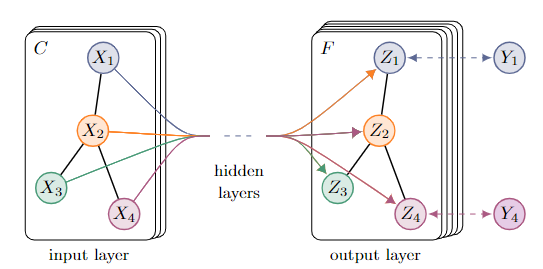
\includegraphics[width=0.55\textwidth]{gcn.png}
    \caption{一阶图卷积神经网络。}
    \label{fig:gcn}
\end{figure}

GCN通过对谱方法做一阶局部近似,实现了一个多层的图卷积神经网络。其中每一个卷积层仅处理一阶邻域信息,通过叠加若干卷积层可以实现多阶邻域的信息传递,但是网络层数如果太深,会出现过平滑(over smoothing)的现象,即每个顶点的输出特征都十分相似,反而造成网络效果变差。尽管GCN经过推导证明了自己是谱方法的一阶近似实现,但是实际上每个卷积层都是在做一次对所有结点的一阶邻域的信息聚合,该方法也架起了谱方法和空间方法之间的一道桥梁。

\mypara{Graph Attention Network} 
继谷歌提出Transformer~\cite{vaswani2017attention}之后,注意力机制(attention mechanism)引起了各领域的研究人员的广泛关注,研究热潮中大家都在尝试结合注意力机制对自己的课题做出进一步探索。Veličković等在2018年提出了图注意力网络~\cite{velivckovic2018graph}。图注意力网络通过注意力机制定义聚合函数,在图注意力网络中,邻接矩阵仅被用来定义相关结点,而关联权重的计算则依赖于结点的特征表达。
\begin{figure}[htb!]
    \centering
    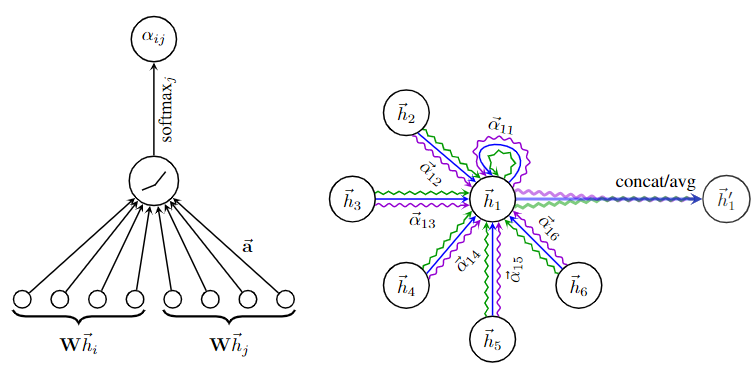
\includegraphics[width=0.70\textwidth]{GAT.png}
    \caption{图注意力网络。}
    \label{fig:GAT}
\end{figure}

图注意力网络每层的结构如图\ref{fig:GAT}所示,图\ref{fig:GAT}左图以结点$i,j$之间的注意力分数并归一化的特征表达作为输入,计算$i,j$之间的注意力分数并归一化,右图描述的是一个结点利用计算出的与周围结点之间的注意力分数将周围结点的表达以加权和的形式聚合到自身。注意力打分和结点$i$表达的更新公式如下
\begin{align}
    &\alpha_{i,j}
    = \frac{
    \exp \left(
    \mathrm{LeakyReLU} \left(
    \boldsymbol{a} \left[ \boldsymbol{Wh}_i
    \Vert \boldsymbol{Wh}_j \right]
    \right) \right)}{
    \sum_{k \in \mathcal{N}_i}
    \exp \left(
    \mathrm{LeakyReLU} \left(
    \boldsymbol{a} \left[ \boldsymbol{Wh} _i
    \Vert \boldsymbol{Wh}_k \right]
    \right) \right)
    } \notag \\
    &\boldsymbol{h}_i =
    \sigma \left(
    \sum_{j \in \mathcal{N}_i}
    \alpha_{i,j} \boldsymbol{Wh}_j
    \right) \label{gat-formula} 
\end{align}
其中,参数$\boldsymbol{W}$矩阵用于完成每个结点的特征维度变换,参数$\boldsymbol{a}$是一个权重参数向量,$\Vert$是拼接操作,$\boldsymbol{h} _i$即为结点$i$的特征表示,$\alpha_{i,j}$表示在参数$\boldsymbol{a}$下计算得到的结点$i,j$间的注意力分数,防止与结点的特征表示混淆,我们在这里用$\sigma$表示非线性激活函数。

此外,作者也效仿Transformer~\cite{vaswani2017attention}中的多头注意力(multi-head attention)机制,图\ref{fig:GAT}中右图里不同颜色就代表不同的注意力头的计算过程(3个注意力头),之后将结果进行拼接或平均,关于拼接和平均的具体公式如下
\begin{align}
    & \mathrm{concat:}\quad 
    \boldsymbol{h}'_i =
    \sideset{}{}{\mathop{\Big \Vert}}_{l=1}^L
    \sigma \left(
    \sum_{j \in \mathcal{N}_i}
    \alpha_{i,j}^{(l)} \boldsymbol{W}^{(l)} \boldsymbol{h}_j
    \right)   \label{gat-concat} \\
    & \mathrm{average:}\quad 
    \boldsymbol{h}'_i =
    \sigma \left(
    \frac{1}{L} 
    \sum_{l=1}^L
    \sum_{j \in \mathcal{N}_i}
    \alpha_{i,j}^{(l)} \boldsymbol{W}^{(l)} \boldsymbol{h}_j
    \right) \label{gat-avg} 
\end{align}
 其中,$L$为所有注意力头的头数,$\alpha_{i,j}^{(l)}$和$\boldsymbol{W}^{(l)}$为标号为$l$的注意力头中对应的注意力分数和变换矩阵。
 


%%%%%%%%%%%%%%%%%%%%%%%%%%%%%%%%%%%%%%%%%%%%%%

% \begin{figure}[htb!]
%     \centering
%     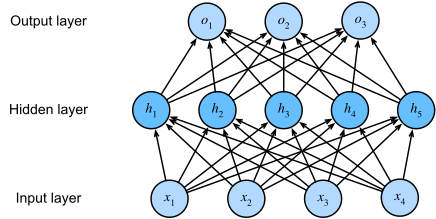
\includegraphics[width=8.6cm,height=4.4cm]{mlp.png}
%     \caption{一个具有一层隐藏层的多层感知器。
%     }\label{fig:mlp}
% \end{figure}

%%%%%%%%%%%%%%%%%%%%%%%%%%%%%%%%%%%%%%%%%%%%%%


%%%%%%%%%%%%%%%%%%%%%%%%%%%%%%%%%%%%%%%%%%%%%%%%%%%%%%%%%%
\section{应用}

图卷积神经网络自提出以来,受到了研究人员的大量关注,主要集中于以下几个领域:网络分析、推荐系统、生物化学、交通预测、计算机视觉、自然语言处理等。图卷积神经网络的应用领域既包括计算机科学、人工智能、信号处理等传统机器学习领域,也包括物理、生物、化学、社会科学等跨学科的研究领域。

徐冰冰等人在去年发表的综述中总结~\cite{徐冰冰2020图卷积神经网络综述}了常见分类,见下表\ref{tab:apply-sum}。
\begin{table}[htbp!]
    \centering
    % \begin{tabularx}{\textwidth}{lXXXXX} 
    \begin{tabularx}{\textwidth}{XXXp{3cm}Xp{5cm}}
    \toprule
        应用领域  &  结点  &  连边  &   应用问题 &  任务 &  相关论文 \\ 
    \midrule
        网络分析 &  用户   &  社交关系  & 用户影响力预测  & 图回归 & DeepInf~\cite{qiu2018deepinf}
        \\ 
                     & 论文 & 引用关系 & 半监督结点分类 & 节点分类 & 
                     GCN~\cite{kipf2016semi},GAT~\cite{velivckovic2018graph},\newline GWNN~\cite{xu2018graph}
                     \\  
    \midrule
        推荐系统 &  用户,商品   &  购买某商\newline 品的可能\newline 性分数  & 用户偏好推荐  & 矩阵补全/ \newline 链接预测 & PinSage~\cite{ying2018graph},RippleNet~\cite{wang2018ripplenet,wang2019exploring},\newline  GraphRec~\cite{fan2019graph}
        \\ 
    \midrule
        生物化学 &  小分子  & 化学键  & 化学功能预测  & 图分类 & 
        Duvenaud等人~\cite{duvenaud2015convolutional},\newline Kearnes等人~\cite{kearnes2016molecular},GAM~\cite{lee2018graph}
        \\ 
        & 蛋白质/\newline 药物 & 相互作用 & 副作用预测 & 链接预测 & 
        Decagon
        \\ 
    \midrule
        计算机\newline 视觉 &  3D点云图   & 距离信息  & 语义分割/\newline 形状分类  & 语义分割 & 3DGNN~\cite{qi20173d},SPG~\cite{landrieu2018large},\newline RGCNN~\cite{te2018rgcnn}
        \\ 
        & 对象 & 对象之间\newline 的关联 & 场景图生成/\newline 视觉推理 & 图生成 & 
        Graph VQA~\cite{teney2017graph},GRM~\cite{wang2018deep}
        \\ 
    \midrule
        自然语言\newline 处理 & 概念实体   & 语义关系  & 知识推理  & 链接预测 & GNN-for-OOKB~\cite{hamaguchi2017knowledge}\\ 
        & 词   & 依赖关系  & 语义角色标注/\newline 抽象含义表达  & 关系提取 & 
        Semantic GCN~\cite{marcheggiani2018exploiting},\newline LSTM+GCN~\cite{marcheggiani2017encoding},C-GCN~\cite{zhang2018graph}
        \\ 
        & 词   & 依赖关系  & 事件提取  & 序列标注 & 
        JMEE~\cite{liu2018jointly},Nguyen等人~\cite{nguyen2018graph}
        \\ 
        & 词   & 共现关系  & 文本分类  & 图分类 & 
        HR-DGCNN~\cite{peng2018large},TextGCN~\cite{yao2019graph}
        \\ 
    \bottomrule
    \end{tabularx}
    \caption{图卷积神经网络应用领域总结表(引自徐冰冰等综述~\cite{徐冰冰2020图卷积神经网络综述})。}\label{tab:apply-sum}
\end{table}

除了上述应用领域之外,在优化求解和程序推断~\cite{khalil2017learning,li2018combinatorial}等任务上,图卷积神经网络都开始被人们使用。由于其可以建模在现实生活中常见的图数据上,并且通过卷积、注意力或消息传播等机制,能够将网络的拓扑结构和结点属性等信息以神经网络进行捕获和建模,因此图卷积神经网络有广泛的应用前景。



%%%%%%%%%%%%%%%%%%%%%%%%%%%%%%%%%%%%%%%%%%%%%%%%%%%%%%%%%%



%%%%%%%%%%%%%%%%%%%%%%%%%%%%%%%%%%%%%%%%%%%%%%%%%%%%%%%%%%




%%%%%%%%%%%%%%%%%%%%%%%%%%%%%%%%%%%%%%%%%%%%%%%%%

\section{小结}\label{sec:Conclusion}

图卷积神经网络是能够较高效地处理图数据的模型,在过去几年受到广泛关注,本文对图卷积神经网络的两种主流方法做了梳理和简单介绍,总结了一些较为经典的模型和方法。

图卷积神经网络方面的工作主要面临着三个挑战:图数据是非欧空间数据,图数据的多样性,图数据规模庞大。

在第\ref{sec:SpectralMethod}节和第\ref{sec:SpatialMethod}节中,我们总结了目前的两类主流方法:谱方法利用图傅里叶变换和卷积定理在谱域定义图卷积,空间方法在结点域定义加权函数再聚合中心结点及其邻居结点的特征。此外,我们还总结了一些经典的图卷积神经网络模型,并且分析了其优缺点,简要介绍了图神经网络适用的应用问题。总的来说,图卷积神经网络已经取得了一定效果,但仍有一些问题需要解决,以使得它在图数据的场景下被充分利用。

% 本次实验中,经过结果分析和参数调整后,5种分类器基本都在各数据集的具体任务上取得了较良好的准确率表现。通过对算法基本原理的整理和重新学习,让我更加深刻地体会到了具体问题具体分析的重要性。面对具体任务首先要了解、分析数据集与相应的任务要求及其内容,对数据集的分布、实际场景中的情况和模式识别任务都要先认识清楚之后,才能更好地利用学习过的基本方法去处理问题。了解应用场景是解决“从哪里来”的问题,分析数据集对应“是谁”的问题,把握具体任务的要求和内容又是回答“到哪里去”问题的过程。模式识别与机器学习不是简单算法的堆积,将其拿过来和数据集挨个配对处理之后比较一下就高枕无忧了,更多时候需要依据任务特点对现有的方法进行一定程度的改变和融合(如使用IBk方法处理Occupancy Detection数据集的过程)。


{
% \small
\normalsize
\bibliographystyle{ieee}
\bibliography{Saliency}
}


% \clearpage
% \section*{附录}\label{sec:appendix}
% 本次作业的实现代码见附件目录下Fisher\_LDA.ipynb和Linear\_SVM.ipynb两个文件,安装Python及Jupyter\;Notebook等所需的库之后打开即可逐个cell运行。

% \end{CJK*}
\end{document}
